% Template LaTeX file for DAFx-11 papers

%------------------------------------------------------------------------------------------
%  !  !  !  !  !  !  !  !  !  !  !  ! user defined variables  !  !  !  !  !  !  !  !  !  !  !  !  !  !
% Please use these commands to define title and author of the paper:
\def\papertitle{The Faust Synthesis ToolKit}
\def\paperauthorA{Romain Michon}
\def\paperauthorB{Julius O. Simith}


%------------------------------------------------------------------------------------------
\documentclass[twoside,a4paper]{article}
\usepackage{dafx_11}
\usepackage{amsmath,amssymb,amsfonts,amsthm}
\usepackage{euscript}
\usepackage[latin1]{inputenc}
\usepackage[T1]{fontenc}
\usepackage{ifpdf}

\usepackage[english]{babel}
\usepackage{caption}
\usepackage{subfig, color}

\setcounter{page}{1}
\ninept

\usepackage{times}
% Saves a lot of ouptut space in PDF... after conversion with the distiller
% Delete if you cannot get PS fonts working on your system.

% pdf-tex settings: detect automatically if run by latex or pdflatex
\newif\ifpdf
\ifx\pdfoutput\relax
\else
   \ifcase\pdfoutput
      \pdffalse
   \else
      \pdftrue
\fi

\ifpdf % compiling with pdflatex
  \usepackage[pdftex,
    pdftitle={\papertitle},
    pdfauthor={\paperauthorA},
    colorlinks=false, % links are activated as colror boxes instead of color text
    bookmarksnumbered, % use section numbers with bookmarks
    pdfstartview=XYZ % start with zoom=100% instead of full screen; especially useful if working with a big screen :-)
  ]{hyperref}
  \pdfcompresslevel=9
  \usepackage[pdftex]{graphicx}
  \usepackage[figure,table]{hypcap}
\else % compiling with latex
  \usepackage[dvips]{epsfig,graphicx}
  \usepackage[dvips,
    colorlinks=false, % no color links
    bookmarksnumbered, % use section numbers with bookmarks
    pdfstartview=XYZ % start with zoom=100% instead of full screen
  ]{hyperref}
  % hyperrefs are active in the pdf file after conversion
  \usepackage[figure,table]{hypcap}
\fi

\title{\papertitle}

%-------------SINGLE-AUTHOR HEADER STARTS (uncomment below if your paper has a single author)-----------------------
%\affiliation{
%\paperauthorA\mbox{ and }\paperauthorB\sthanks{CCRMA visiting researcher from Saint \'Etienne University, France, supported by the ASTREE Project}}
%{\href{https://ccrma.stanford.edu/\~{}jos/}{Center for Computer Research in Music and Acoustics}\\ (CCRMA) Stanford University \\ Palo Alto, CA 94305, USA\\
%{\tt \href{mailto:jos|rmichon@ccrma.stanford.edu}{jos@ccrma.stanford.edu}}
%}

\twoaffiliations{
\paperauthorA,\sthanks{CCRMA visiting researcher from Saint \'Etienne University, France, supported by the ASTREE Project}}
{\href{http://ccrma.stanford.edu/~rmichon}{CIEREC, EA 3068} \\ Universit� Jean
  Monnet \\ F-42023, Saint-Etienne, France \\
{\tt \href{mailto:rmichon@ccrma.stanford.edu}{rmichon@ccrma.stanford.edu}}
}
{\paperauthorB,}
{\href{https://ccrma.stanford.edu/\~{}jos/}{Center for Computer Research in Music and Acoustics}\\ (CCRMA) Stanford University \\ Palo Alto, CA 94305, USA\\
{\tt \href{mailto:jos@ccrma.stanford.edu}{jos@ccrma.stanford.edu}}
}
%-----------------------------------SINGLE-AUTHOR HEADER ENDS------------------------------------------------------


\begin{document}
% more pdf-tex settings:
\ifpdf % used graphic file format for pdflatex
  \DeclareGraphicsExtensions{.png,.jpg,.pdf}
\else  % used graphic file format for latex
  \DeclareGraphicsExtensions{.eps}
\fi

\maketitle

\begin{abstract}
The Faust-STK.

\end{abstract}

\section{Introduction}\label{sec:intro}

\section{Waveguide Models}\label{sec:waveguideModels}

Waveguide synthesis was created by Julius O. Smith during the
eighties \cite{waveGuide}. It is based on a modified version of the
Karplus-Strong algorithm \cite{KS} that makes it possible to model any
kind of strings, bores or vibrating structures with a network of delay
lines and filters. Waveguide instruments appears to be very suitable to be implemented with
the FAUST language mainly because of their ``stream like''
architecture.   

The following instruments based on the waveguide synthesis technique were implemented in the {\it Faust-STK}:

\begin{itemize}
\item two clarinets;
\item two flutes;
\item one saxophone;
\item two models of brass instrument;
\item one iron plaque;
\item one wooden plaque;
\item a tibetan bowl;
\item a glass plaque.
\end{itemize}

A brief overview of these models is done in this section.

\subsection{Wind Instruments}

Algorithms used in the {\it Faust-STK} are almost all based on
instruments implemented in the {\it Synthesis ToolKit} and the program
{\it SynthBuilder}. Although, it is important to observe that some of
them were slightly modified in order to adapt them to the FAUST semantic.

Despite the fact that we used as often as possible functions already
defined in the default FAUST libraries to build our models, we needed
most of the time to write our own filters in order to be able to use the
parameters from the {\it STK} classes and the {\it SynthBuilder}
patches. All those functions were put in file called
\texttt{filter.lib}.

\subsubsection{Flutes}

\subsubsection{Clarinets}

\subsubsection{Saxophone}

\subsubsection{Brass Models}

\subsubsection{Other Wind Instrument Models}

\section{Piano Synthesis in Faust} 

\subsection{Find a Title}

A {\it SynthBuilder} patch implementing a commuted piano \cite{commutedPiano} has been
written in the late nineties at Stanford's CCRMA. This patch was partly
ported in 2006 by Stephen Sinclair at McGill University in the {\it
  Synthesis ToolKit} \cite{pianoSTK}. A big part of his work consisted
in extracting the values for each parameters from the {\it
  SynthBuilder} patch to store them in a set of C++ functions. We
reused them to build our FAUST commuted piano version by using the
{\it foreign function} mechanism as described is section \ref{}.

In this piano model, the keyboard is splited in two part which use a
different algorithm. Indeed, the tones
below {\it E6} use the commuted waveguide technique while tones above
or equal to {\it E6} use a serie of biquad filters to generate the
sound (figure \ref{fig:piano}).   

\begin{figure}[ht]
\begin{center}
        \framebox{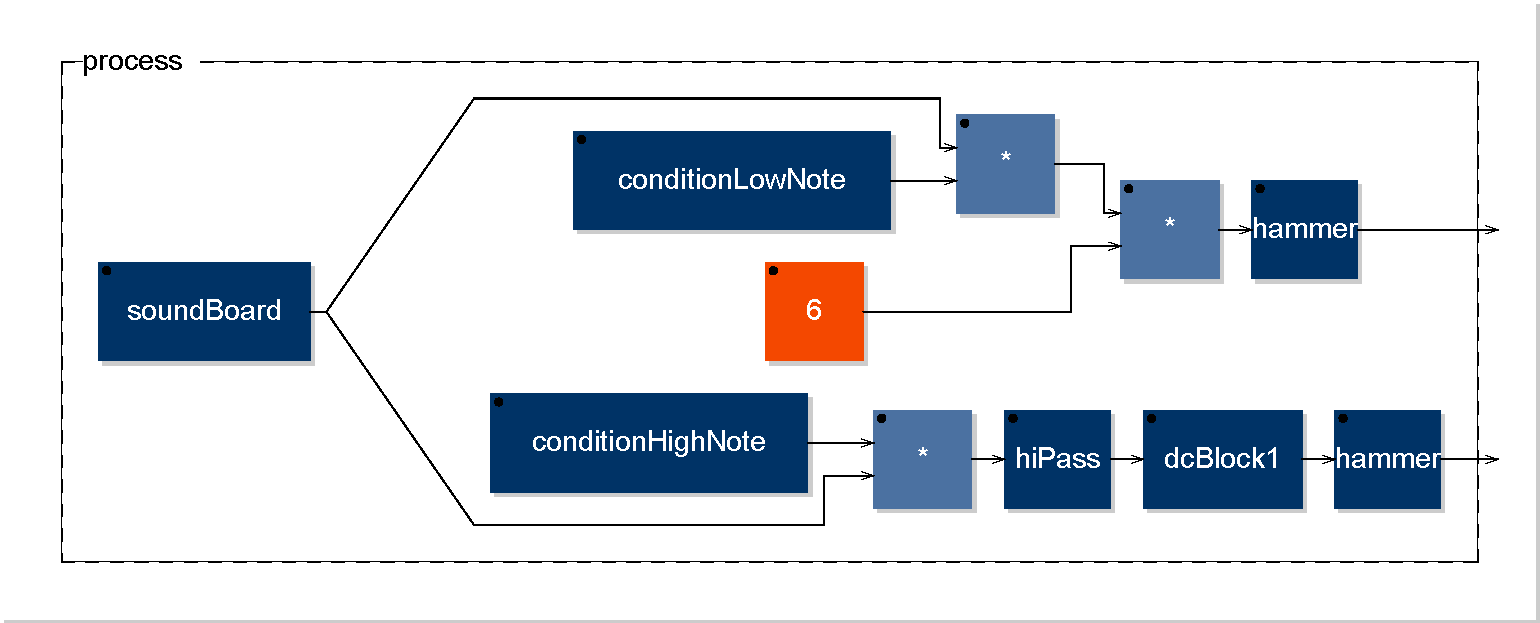
\includegraphics[width=\columnwidth]{fig/piano1.pdf}} \\
        \hspace{2cm}
        \framebox{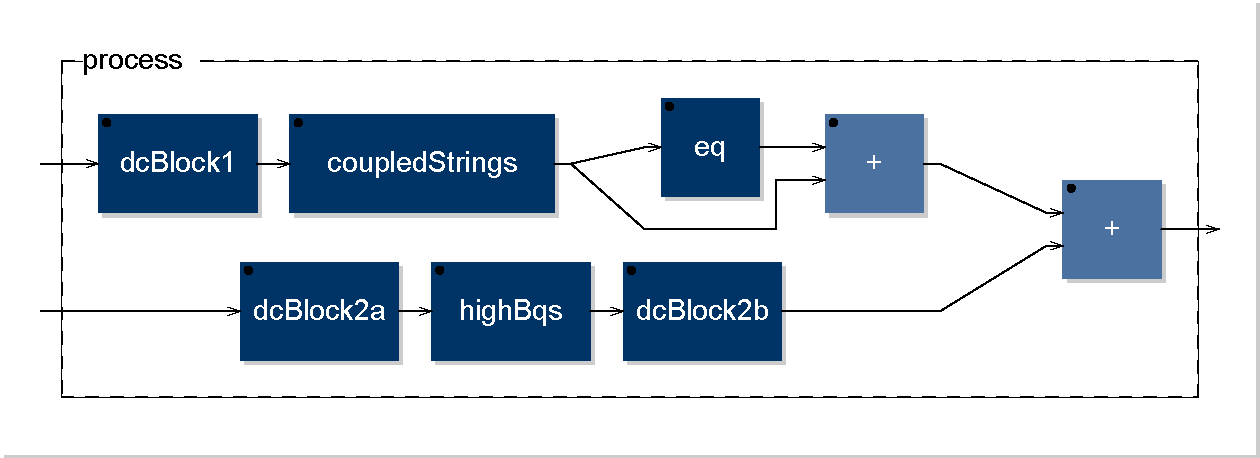
\includegraphics[width=\columnwidth]{fig/piano2.pdf}}
\caption{{\it Commuted piano algorithm drawn by FAUST using
    faust2svg. The upper figure is the beginning of the model and the
    lower figure the end.}}
\label{fig:piano}
\end{center}
\end{figure}

The current FAUST version of the commuted piano is not a polyphonic
instrument. However, the {\it faust2pd} program developed by Albert
Graef \cite{faust2pd} makes it possible to automatically produce {\it PureData}
patches that implement polyphonic synthesizers based on FAUST generated
PD-plug-ins. They can then be controlled via MIDI or OSC directly in
PureData.    

\begin{figure}[ht]
\begin{center}
        \framebox{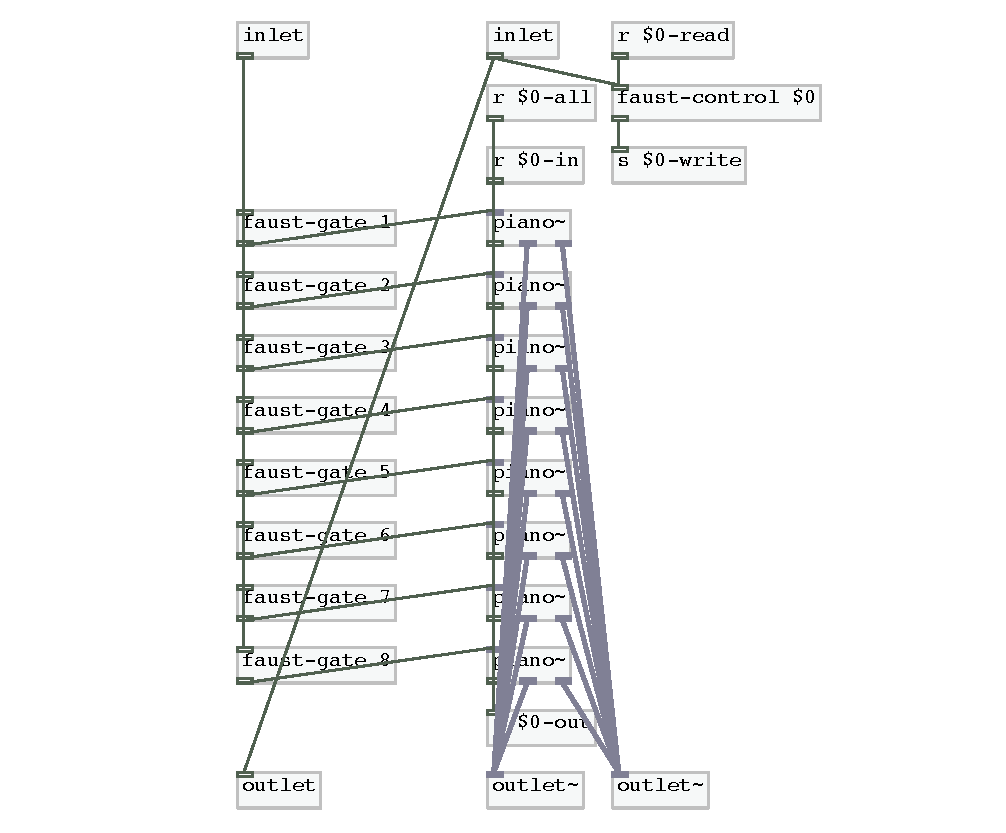
\includegraphics[width=\columnwidth]{fig/pianoPatch.pdf}}
\caption{{\it Synthesis part of the PureData polyphonic sub-patch
    generated with faust2pd from ``piano.dsp''. In the current case, a
  height voices polyphony synthesizer is implemented so
  piano$\sim$.dsp is called height times.}}
\label{fig:pianoPatch}
\end{center}
\end{figure}

\section{Optimization and Performances}

\subsection{File size}

Digital signal processing algorithms can be expressed very shortly in
FAUST. The gain in term of code size with C++ or even matlab
implementation is most of the time very significant. Thereby, we tried
to make the {\it FAUST-STK} algorithms as concise and readable as
possible.

It would be very hard and inaccurate to compare the raw C++ and
FAUST codes together as most of the physical models were implemented
in the {\it Synthesis ToolKit} with several spread out functions that
are most of the time strewn in different files. Moreover, these
functions also contains informations that are not related to the
algorithm itself.

Nevertheless, we were able to carry out such a comparison as a rough
guide. We took into account in FAUST as in C++ the implementation of the
algorithm itself and the line of codes concerning parameters
handling. 

The result of this comparison can be seen in table \ref{tab:nblines}. Once again, even if its results are certainly arguable, it
shows very well how FAUST is efficient in reducing the code
size. 

\begin{table*}[ht]
\begin{center}
\begin{tabular}{c c c c c c c}
\hline
\hline
FAUST file & C++ code & FAUST code & Size gain for & C++ code & FAUST code
& Size gain for\\
name & nb of declarations & nb of declarations & nb of lines & nb of lines & nb of
lines & nb of lines\\
\hline
blowBottle.dsp  & 74 & 30 & {\bf 59.5\%} & 237 & 54 & {\bf 77.2\%} \\
blowHole.dsp & 131 & 66 & {\bf 49.6\%} & 373 & 104 & {\bf 72.1 \%} \\
bowed.dsp &  92 & 45 & {\bf 51.1\%} & 274 & 69 & {\bf 74.8\%} \\
brass.dsp & 90 & 36 & {\bf 60\%} & 272 & 63 & {\bf 76.8\%} \\
clarinet.dsp & 78 & 35 & {\bf 55.1\%} & 255 & 60 & {\bf 76.5\%} \\
flutestk.dsp & 109 & 43 & {\bf 60.6\%} & 309 & 70 & {\bf 77.3\%} \\
modalBar.dsp * & 63 & 37 & {\bf 42.3\%} & 217 & 78 & {\bf 64\%} \\
saxophony.dsp & 98 & 42 & {\bf 57.1\%} & 308 & 69 & {\bf 77.6\%} \\
sitar.dsp & 57 & 25 & {\bf 56.1\%} & 193 & 42 & {\bf 78.2\%} \\
bars * & 164 & 35 & {\bf 78.7\%} & 396 & 70 & {\bf 82.3\%} \\
voiceForm.dsp * & 121 & 65 & {\bf 46.3\%} & 325 & 109 & {\bf 66.5\%} \\
piano.dsp * & 292 & 158 & {\bf 45.9\%} & 750 & 246 & {\bf 67.2\%} \\
\hline
\end{tabular}
\end{center}
\caption{{\it Comparison of the code size of the STK object's C++ code
    with the FAUST code from FAUST-STK. The number of declarations was
    calculated in both cases by counting the number semicolon in the
    code. In the case of the
    instruments where the file name is followed by the
  * sign, parameters data-bases were not taken into account.}}
\label{tab:nblines}
\end{table*}

\subsection{CPU load}

The FAUST compiler optimizes the efficiency of its generated C++
code. Thus, we tried to compare for some models the CPU load between
{\it PureData} plug-ins created using the {\it stk2pd}\footnote{{\it
    stk2pd} is a program that was developed created at Stanford's
  CCRMA by M. Gurevich and C. Chafe. It converts any C++ code from the {\it
  STK} into a plug-in for {\it PureData} \cite{stk2pd}.} program with
PD plug-ins generated by FAUST using the {\it PureData} architecture
file.

In both cases, PD plug-ins were compiled in 32bits and the signal
processing is scalar. Tests were carried out on a MacBook Pro with the
following configuration:
\begin{itemize}
\item processor: 2.2 GHz Intel Core 2 Duo;
\item RAM: 2GBytes DDR2.  
\end{itemize}

Results of this comparison can be seen in table \ref{tab:computationalTest}.

\begin{table}[ht]
\begin{center}
\begin{tabular}{c c c c}
\hline
\hline
FAUST file & STK & FAUST & Difference \\
name &  \\
\hline
blowBottle.dsp  & 3,23 & 2,49 & 22,91 \\
blowHole.dsp & 2,70 & 1,75 &  35,19\\
bowed.dsp &  2,78 & 2,28 & 17,99 \\
brass.dsp & 10,15 & 2,01 & 80,20 \\
clarinet.dsp & 2,26 & 1,19 & 47,35 \\
flutestk.dsp & 2,16 & 1,13 & 47,69 \\
saxophony.dsp & 2,38 & 1,47 & 38,24 \\
sitar.dsp & 1,59 & 1,11 & 30,19 \\
tibetanBowl.dsp & 5,74 & 2,87 & 50 \\
\hline
\end{tabular}
\end{center}
\caption{{\it Comparison of the performances of PureData plug-ins
    using the STK C++ code with their FAUST generated equivalent. Values
  in the ``STK'' and ``FAUST'' columns are CPU loads in percents. The
  ``difference'' column give the gain of efficiency in percents.}} 
\label{tab:computationalTest}
\end{table}

\section{Conclusions}
This template can be found on the conference website.
For changing the number of author affiliations (1-4), uncomment the corresponding regions in the \texttt{DAFx09\_tmpl.tex} file.
Please, submit full-length papers (max.~8 pages both oral and poster presentations).
Submission is fully electronic and automated through the Conference Web Submission System.
DO NOT send us papers directly by e-mail.

\section{Acknowledgments}
Many thanks to the great number of anonymous reviewers!

%\newpage
\nocite{*}
\bibliographystyle{IEEEbib}
\bibliography{ref} % requires file template.bib

\section{Appendix: Margin Check}
\end{document}
